\chapter{Implementation}


Each iteration of the project will be described




\section{Client Implementation}
\subsection{Mapping}
The first iteration focused on the central component of the application, the map. It was vitally important that an appropriate mapping solution was used.

\subsubsection{Google}
Google provides a simple, easy to use interface to their own maps making it the obvious choice for any Android application. Their maps are accurate, up-to-date and very detailed.

Unfortunately there are a number of restrictions in place stopping their use in a number of situations. The most relevant of which is that they can not be used in an application that is not freely available to the public. Therefore restricting it's use in a paid-for application, such as MapWars may become. As the future of the application is uncertain it seemed desirable to steer clear of as many possible restrictions as possible. For this reason it was important to find a comparable alternative.

\subsubsection{OpenStreet Map}
OpenStreet map is an INSERT DESCRIPTION OF OSM HERE. It's growing popularity means that INSERT STATS ABOUT AREAS COVERED. With an acceptable level of detail combined with it's open SOMETHING(ethos?) made it the next most obvious source.

OSM has an API that allows it to be easily embedded into webpages but no native android SDK. A number of 3rd party libraries are available. The most complete and popular is that provided by MapQuest.

MapQuest are a mapping company that combines proprietary data and OSM data to create their own maps. They offer an Android SDK that gives you the option of which tile source to use. There are obviously restrictions to the proprietary data but if you opt for the free tiles then the same license is used as with OSM. The Android SDK available was designed to mirror the API available for the Google Map SDK. This made swapping out the Google Maps code and replacing it with the MapQuest code was trivial and problem free.

At the point in time of implementing MapQuest the design had called for the option to switch between satellite and road maps. MapQuest's main drawback, and more widely OSM itself, was it's lack of detail. The level of zoom supported was a number of levels less than that of Google Maps. These extra zoom levels would have made unit manipulation easier on smaller devices. Satellite images were the main concern as they were not available at the level of zoom required to make game play comfortable.

MapQuest was used as the mapping solution for a large portion of development and offered a stable platform. Once more of the functionality was in place user testing presented a number of problems with the map tiles being used. Most significant of which was a difficulty in being able to locate units among the details presented with the map. The sprites and colours being used to represent units were experimented with but none were clearly visible. The problem was with the design of the tiles being used and not necessarily the zoom levels present, although this may have helped alleviate the problems.

\subsubsection{MapBox}
One option available was to use a tile creator and host the map tiles on a server. This would be a costly and difficult solution to the problem. Hosting tiles is not a trivial task and require large amounts of storage and bandwidth.

MapBox offer beautiful hosted tiles. They also have their own software called TileMill which allows the creation of bespoke tiles based on any data source which can then be hosted and distributed via their network. TileMill was based on a CSS style syntax allowing you to customise any visual aspect, from line widths, colours, strokes. It also had the ability to import data from any source giving the ability to build up rich tiles with as much detail as required. For MapWars only the most basic detail was required while using a simple colour pallet. The idea was to make any unit stand out against the map while still presenting all the information required to orientate the user with their surroundings. 

Tiles could be loaded from MapBox using a standard URI syntax used by the most tile vendors. This allowed it to integrate easily into any mapping framework.All that was needed was an SDK that allowed custom tile sources. Such functionality was found in OSMDroid. Like with MapQuest, OSMDroid followed the same pattern as Google Maps allowing it to be easily placed into the application without only one substantial problem. OSMDroid was missing one function that was supported by both Google Maps and MapQuest. These function was key in selecting units so had to be reimplemented ... which was not difficult but took time. Assumption was made it would be as effortless as the previous transition. After integration was complete plugging in the URI to my generated tiles was simple and worked straight of the bat.

MapBox did not offer satellite imagery but the beauty and simplicity of the maps being used made up for this. It was also decided that the complexity of such maps would just present the same images as found with the default OSM tiles. Satellite images could always be added to OSMDroid by simply finding a tile source and using that and would have no affect on the functionality of the application. 


\subsection{Location}
Detecting the users location accurately is fundamental and is used directly in controlling game play throughout the game.

There are a number of difficulties presented when trying to accurately determine a users location. Firstly is the array of different providers available, each with their own unique characteristics, advantages and disadvantages.

The network location provider uses the phones network connections to try and determine the users location. If they are connected via Wi-Fi the SSID (Service Set Identifier) is queried against Google's database of known SSID's, returning a location. This database is built by crowd sourcing data from Android handsets. When enabling location services on an Android device the following messages is displayed, \"Allow Google's location service to collect anonymous location data\". Periodically the users location data from GPS, Cell-ID and Wi-Fi is broadcast along with details about available Wi-Fi connections to Google. This data tends to be fairly accurate, however when not connected to Wi-Fi the network location provider returns a location based upon Cell-ID. This technique identifies the mobile network providers cell the users is in. The location of each Cell-ID can be located so an estimated can be produced for the users location. Unfortunately cells can be very large making this method very inaccurate, however this tends to be around 1km and even less within rural locations\cite{1377314} making it acceptable for this application.

When taking location data from a variety of sources it is critical to have a process to determine which is the most accurate to the users current location. The developers guide on location strategies\cite{location} was an ideal resource to understand how each different provider worked and ultimately how to combine them to produce the best outcome. Each provider will gather data at different times and to a different level of accuracy. Whenever this data is processed a judgement needs to be made into whether this is more reliable than the currently known location. This was made based on its accuracy and age.

The process used to determine the most accurate location was adapted from an example provided in the developer guide. As shown in figure \ref{fig:location} each new location is compared against different aspects of the previously known location to decide if it is more or less accurate. If no previous location has been noted then the new data is taken to be the most accurate. If there has been a previous location the new location is only used if it is significantly newer else, if it is not significantly older, the accuracy of the two sources are compared. Each time a new location is received it comes with an estimated accuracy. This accuracy is measured in meters and is defined as the radius of 68\% confidence\cite{location_accuracy}. Meaning that there is a 68\% chance that the user is located within a circle with a radius of the accuracy, mapped around the supplied location.

\begin{figure}[H]
  \centering
   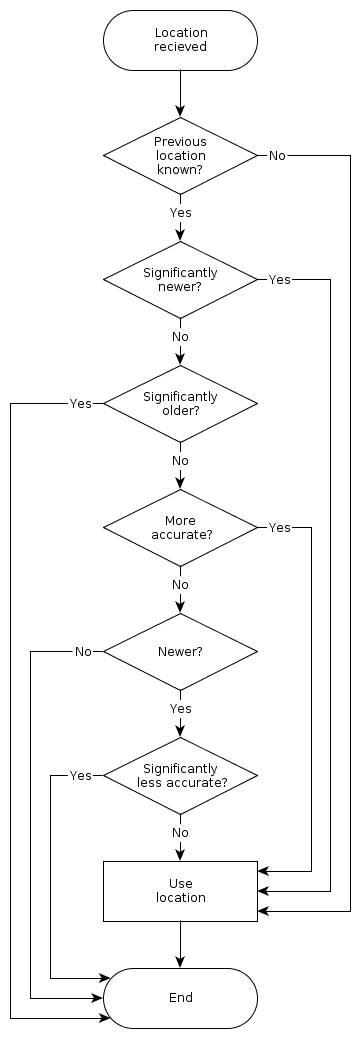
\includegraphics[height=0.9\textheight]{Images/diagrams/location.png}
  \caption{Location flowchart}
  \label{fig:location}
\end{figure}


\subsection{GUI}
9-patch
Different layouts for different devices
Different orientation for different devices


\subsection{Communication}
PUSH/PULL
XML/JSON

\subsection{Units}



\section{Server Implementation}

\subsection{Echo}

\subsection{Units}

\subsection{Storage}

\subsection{AI}
